\documentclass[12pt]{article}
\usepackage[utf8]{inputenc}
\usepackage[english]{babel}
\usepackage{graphicx}
\begin{document}
\begin{titlepage}
\centering



\vspace{1cm}

{\Large \bfseries E-Commerce and Web Engineering Lab CSE-4114}

\vspace{1cm}
{\Large \bfseries Online Tutor}

\vspace{2.5cm}
{\large \bfseries Submitted By}

\vspace{0.5cm}
{\large Dewan Tariq Hasan (AE - 10)}

{\large Md. Aminul Islam (AE - 122)}

{\large 4th year,1st semester}

{\large Group ID : 2018EWE06\vspace{1cm}}

{\large \bfseries Submitted To\\}
\vspace{0.5cm}
{\large Md. Mahmudur Rahman\\Lecturer,Dept. of CSE\\University of Dhaka}
\\
\vspace{1cm}
{\large 6th May, 2018}
\vspace{1cm}
\vfill


{\large \bfseries Department of Computer Science and Engineering}

{\large \bfseries University of Dhaka}
\end{titlepage}
%
\tableofcontents
\newpage
%
%
\section{Introduction}
\par The exponential growth of internet data traffic has led to the emergence of online learning. Nowadays students of various level can get information and reading materials from millions of sites in internet. So, internet is an important platform to learn. 
%  
\vspace{0.5cm}
%
\par In Bangladesh, many of students have lack of proper guidelines about their studies. Our OnlineTutor site is to help them through online. They can get their reading materials and can appear practice problems. 
%
%
\vspace{0.5cm}
%
%
\section{Description}
\par Our website is consist of several different pages.Different page's functionality is different. The short description of pages are here: 
%
%
\subsection{Home}
\par Home page is the main page or starting page of our site. It describes and shows some our courses. From this page instructor or student can have an overview of the site. A naive user can get a concept of this page. It contains a navigation bar top of the page.This navigation bar some important pages link of the the site.
%
\subsection{Sign up and Log in}
To use this site interactively an instructor or student have to sign up to this site. There is a sign up button on the navigation of the site. While doing sign up a user have to ensure that he is instructor or student. As well as he have to put his name,user id email, date of birth and a valid password. For further log in a user have to put his user id as well as password. By creating an id in this site a user(Instructor of Student) creates his own profile page that contain his enrolled or created courses and some personal information.
% 
\subsection{Course}
\par Course page describes different courses. By clicking a course from the drop down block of left side one user(Instructor of Student) can see the course page. That particular course page shows different contents of the course as a drop down block of left side. By clicking one content a user can read the content right of the page. 

\subsection{Instructor}
\par An instructor is an user who instructs some courses. He can provide course content and set quizzes.The courses that an instructor instructed is added to 'My courses' of his profile.
%   
\subsection{Student}
\par A student is an user who can enroll a particular course to learn.The courses that a student enrolled is added to 'My courses' of his profile. To get this advantages a student have to log in first.  
%
%
\section{Objectives}
\begin{itemize}
    \setlength{\itemsep}{1pt}
    \setlength{\parskip}{0pt}
    \setlength{\parsep}{0pt}
    \item To provide education through internet
    \item To provide place independent learning
    \item  To create a platform for giving and receiving knowledge
    \item To create a platform expert instructor
    \item To ensure proper learning for every level of student
    \item To digitize the learning 
\end{itemize}
%
 
\section{Database Design}
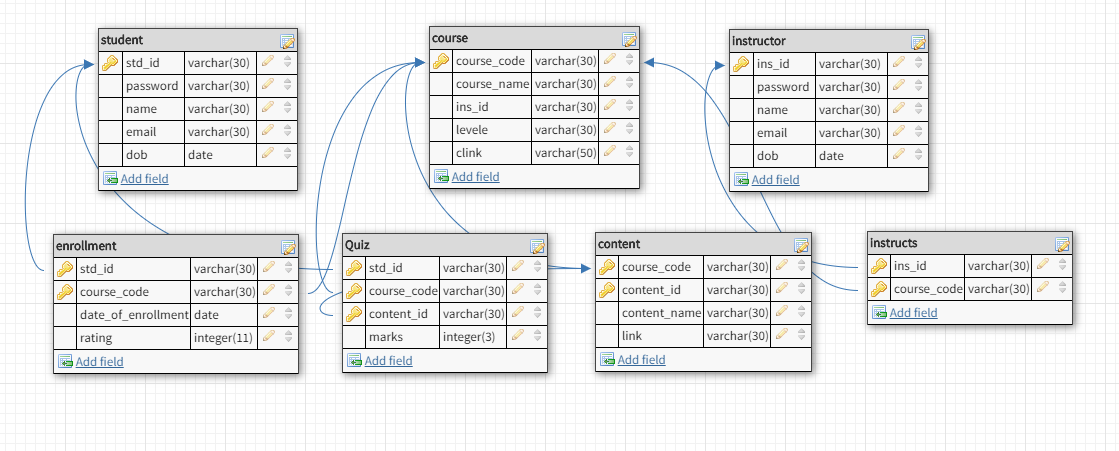
\includegraphics[scale=0.55]{database.PNG}
\section{Platform}
\begin{itemize}
    \setlength{\itemsep}{1pt}
    \setlength{\parskip}{0pt}
    \setlength{\parsep}{0pt}
    \item HTML 5
    \item CSS 3
    \item PHP 7.2
    \item MySQL 5.7 
 
\end{itemize}
%
%
\section{Main features}
%
\subsection{For Instructor}
\par To interact with this site as an instructor, someone first need sign up to this site with information like name, email, user id, date of birth etc. Then an instructor will see his profile page. On that page he will also watch his courses(named by 'My Courses') that he instructs. For the first time he has to create a course by clicking on 'Add new course'. Further he can add content under that course by same procedure. An instructor can instruct one or more course.
%
\subsection{For Student}
\par To learn from this site as a student, someone also need to sign up to this site with information like name, email, user id, date of birth etc. Then a student can see his profile page where he also watch his courses(name by 'My Courses') that he enrolled. For the first time a student has to choose a course from 'Courses' page that he want to enroll. Then he can watch that particular course on his profile in 'My Courses' section. A student can learn course content by visiting the course pages. 
%
%
\section{Conclusion}
\subsection{Summary}
\par Our work is to design an educational site to facilitate learning for students as well as to give opportunity to expert instructors. We have tried to build an interactive site where student of various level get opportunity to educate themselves. A database has designed for this site that store all the data of instructor, student and contents.
%   
\subsection{Problem Faced}
\par The journey to build a website was to easy for us. While building this site we faced various challenges. First, we built the database for the site that was the most challenging part of the work. We have reviewed the database for several times. After that, we had to familiar with the HTML, CSS and PHP language. Another challenging part was enrollment portion to any course for a student. 
%
\subsection{Future Plan}
\par We have some plan for further improvement of this site. In future, we planned to build a evaluation system for proper learning of students. On that improvement an instructor can provide different questions for a particular content that he provide. This questions will be saved to database. While a student wish to take an exam on a particular content, the saved questions will be shown dynamically.
%
\vspace{0.5cm}
%
\par  In future, we want to build this site as an e-commerce site. On that improvement an instructor can provide his own created contents in return of money.For that, we want to build a payment system.
%
\vspace{0.5cm}
%
\par We want to improve some other things of this site, such as instructor and student profile, more interaction with the site as well as more beautiful to watch this site.

\end{document}



